\tableofcontents
\clearpage

\section{Эксперимент №1}

На рисунке \ref{img:1} представлен результат эксперимента.

\begin{figure}[H]
	\caption{График эксперимента 1}
	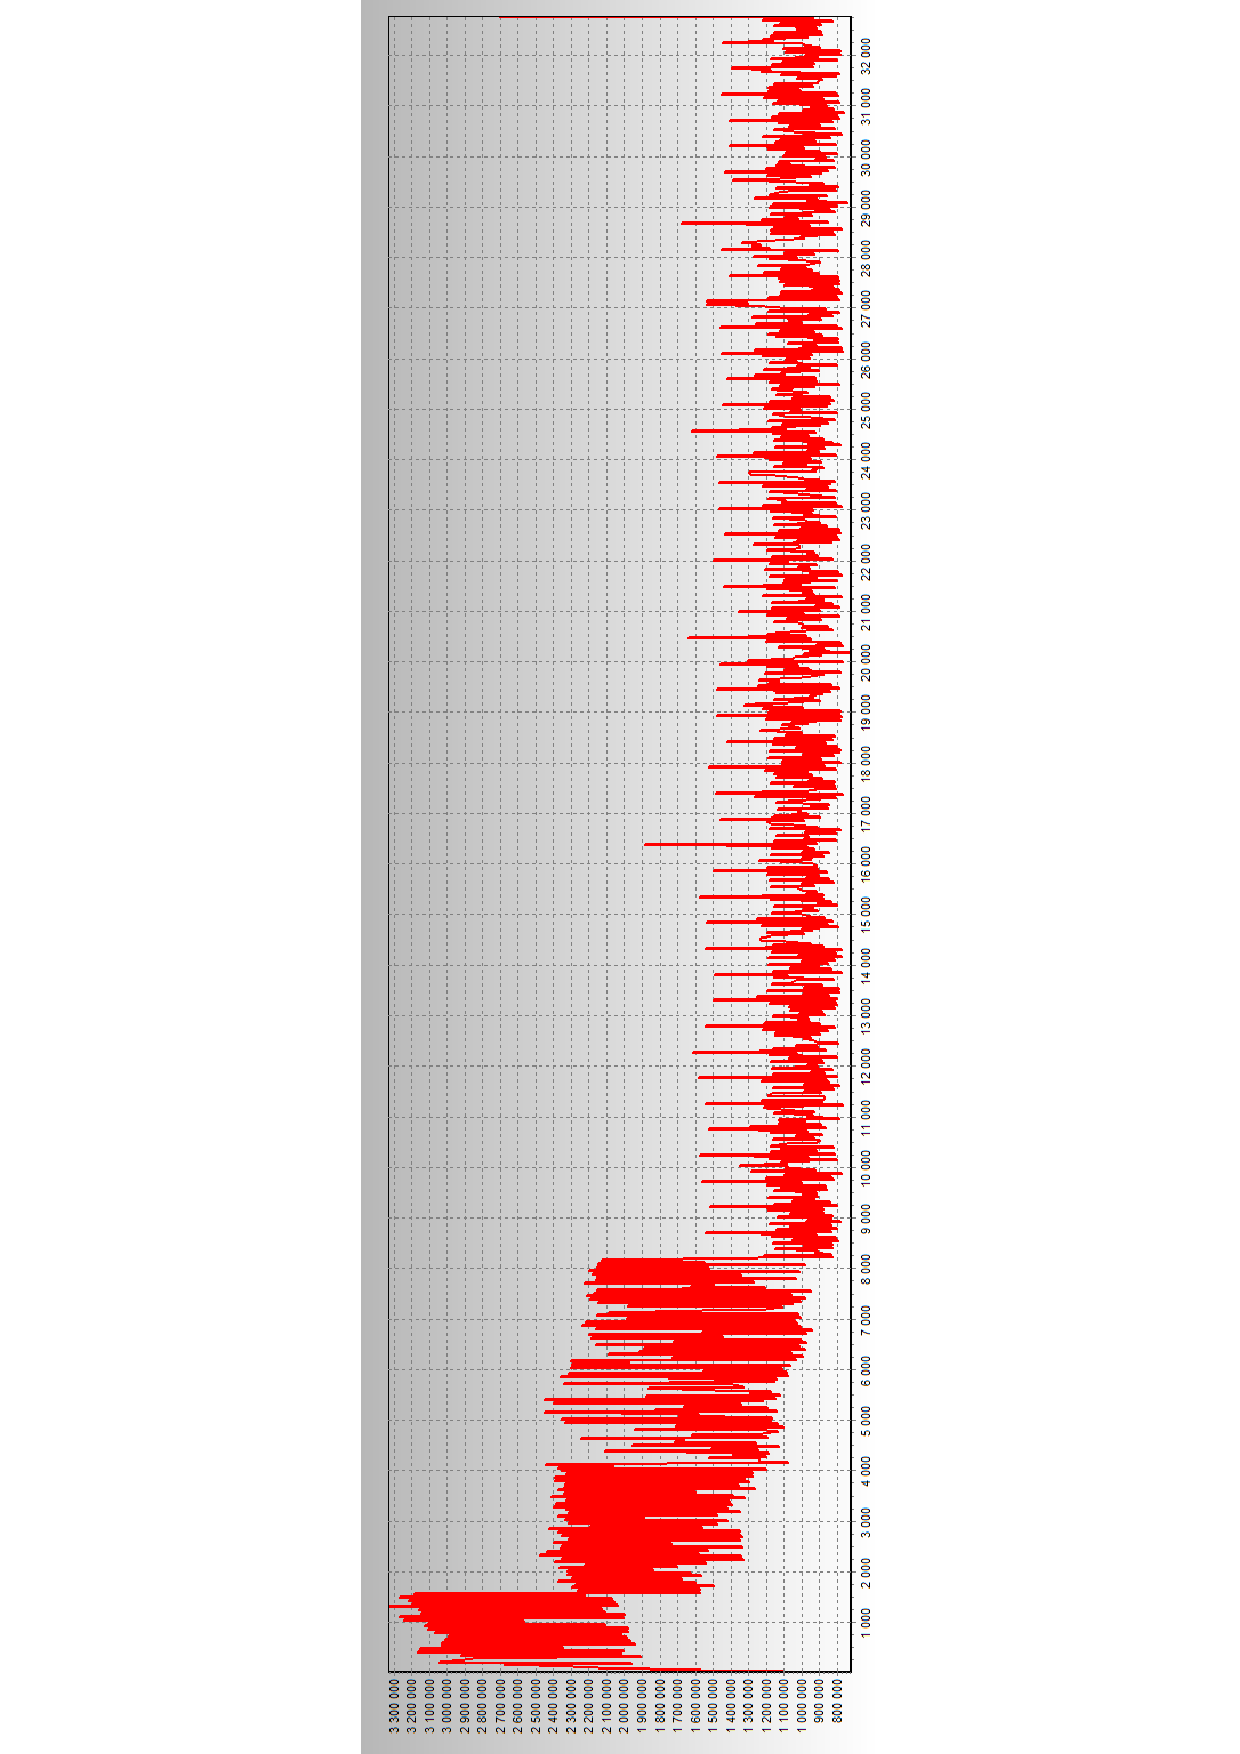
\includegraphics[width=0.7\textwidth, angle=90]{img/1.pdf}
	\label{img:1}
\end{figure}

Точка 1 равна 1024, точка 2 --- 4096.
Число банков --- $1024/128 = 8$.

\subsection*{Вывод}

Память неоднородна, она расслоена. При шаге чтения больше т2 количество тактов практически не меняется. 

\section{Эксперимент №2}

На рисунке \ref{img:2} представлен результат эксперимента.

\begin{figure}[H]
	\caption{График эксперимента 2}
	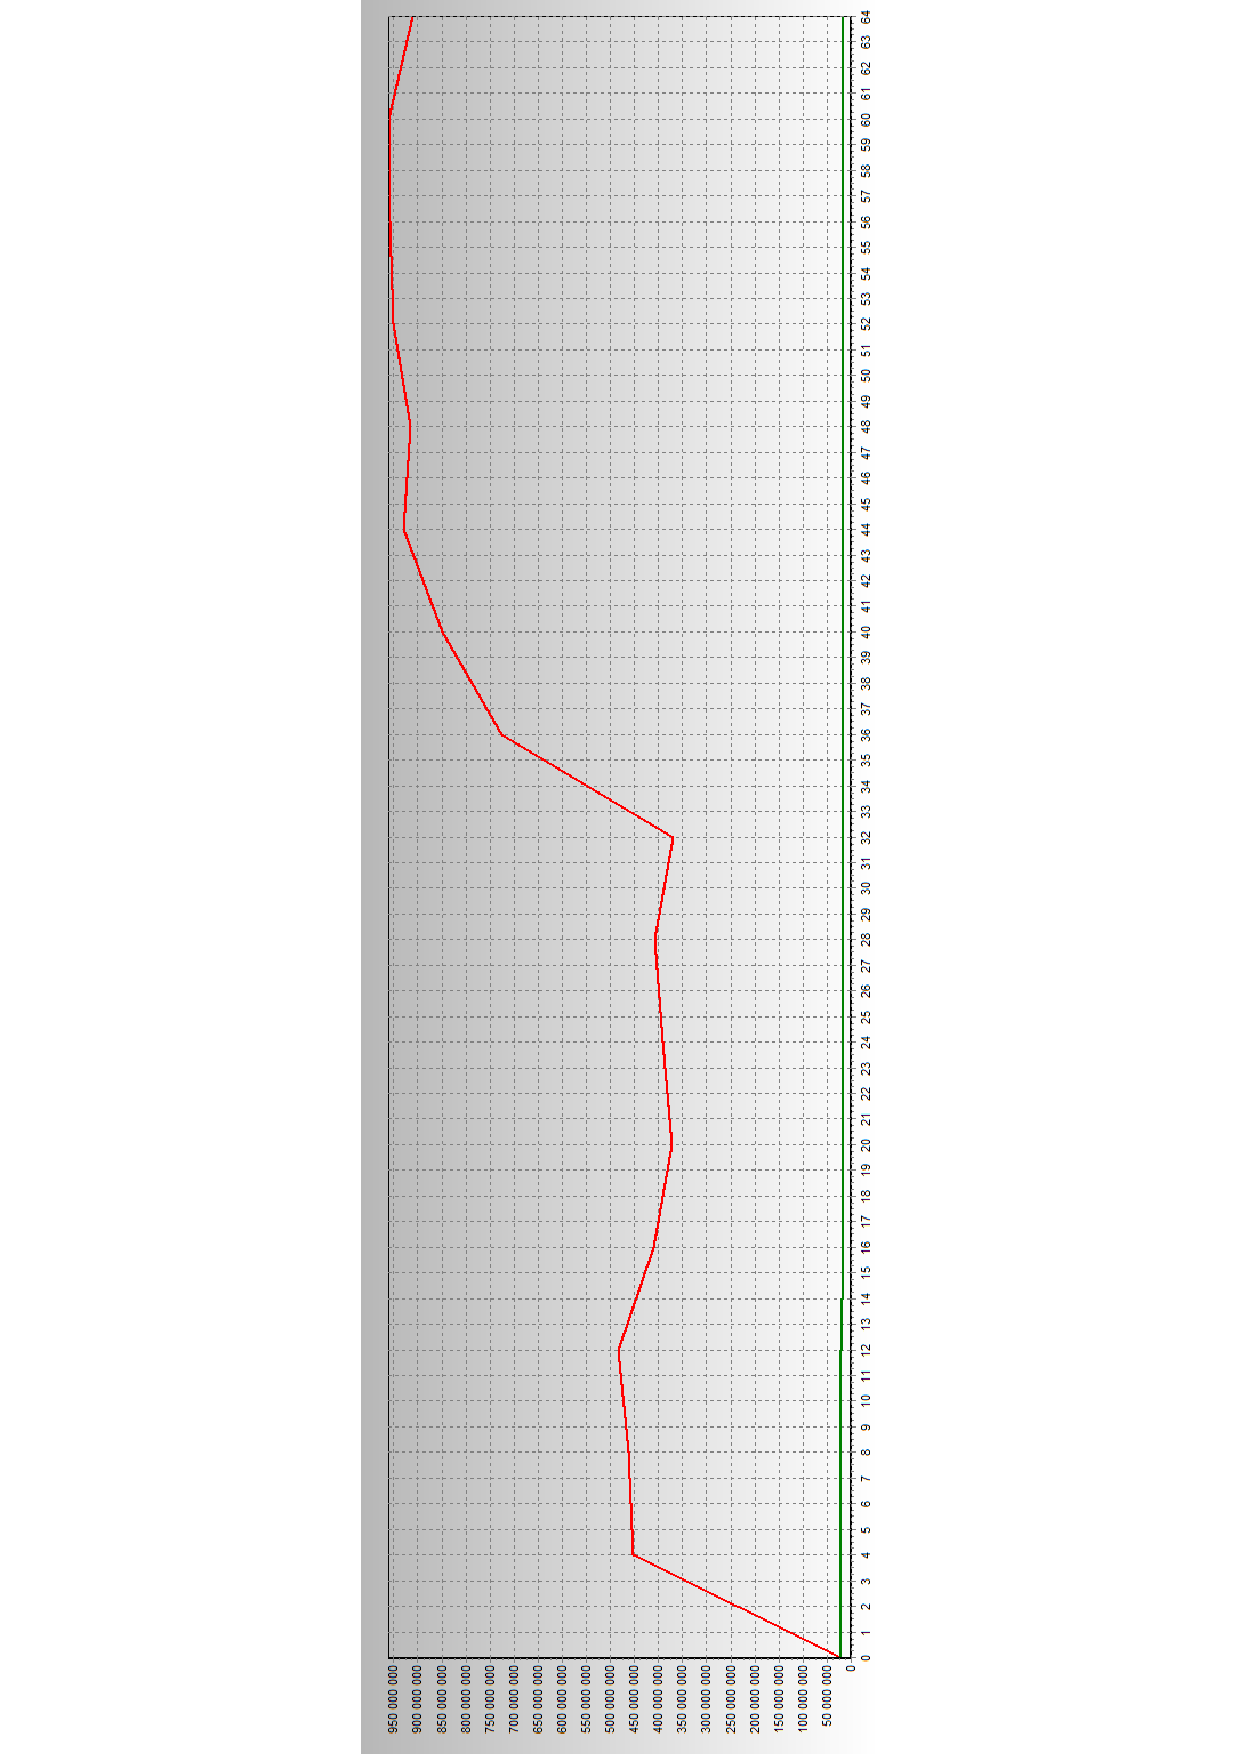
\includegraphics[width=0.7\textwidth, angle=90]{img/2.pdf}
	\label{img:2}
\end{figure}

При большой фрагментации списка время выполнения растет.

\subsection*{Вывод}

Вычислительная машина не предназначена для обработки ссылочных структур, а предназначена для обработки векторных.

\section{Эксперимент №3}

На рисунке \ref{img:3} представлен результат эксперимента.

\begin{figure}[H]
	\caption{График эксперимента 3}
	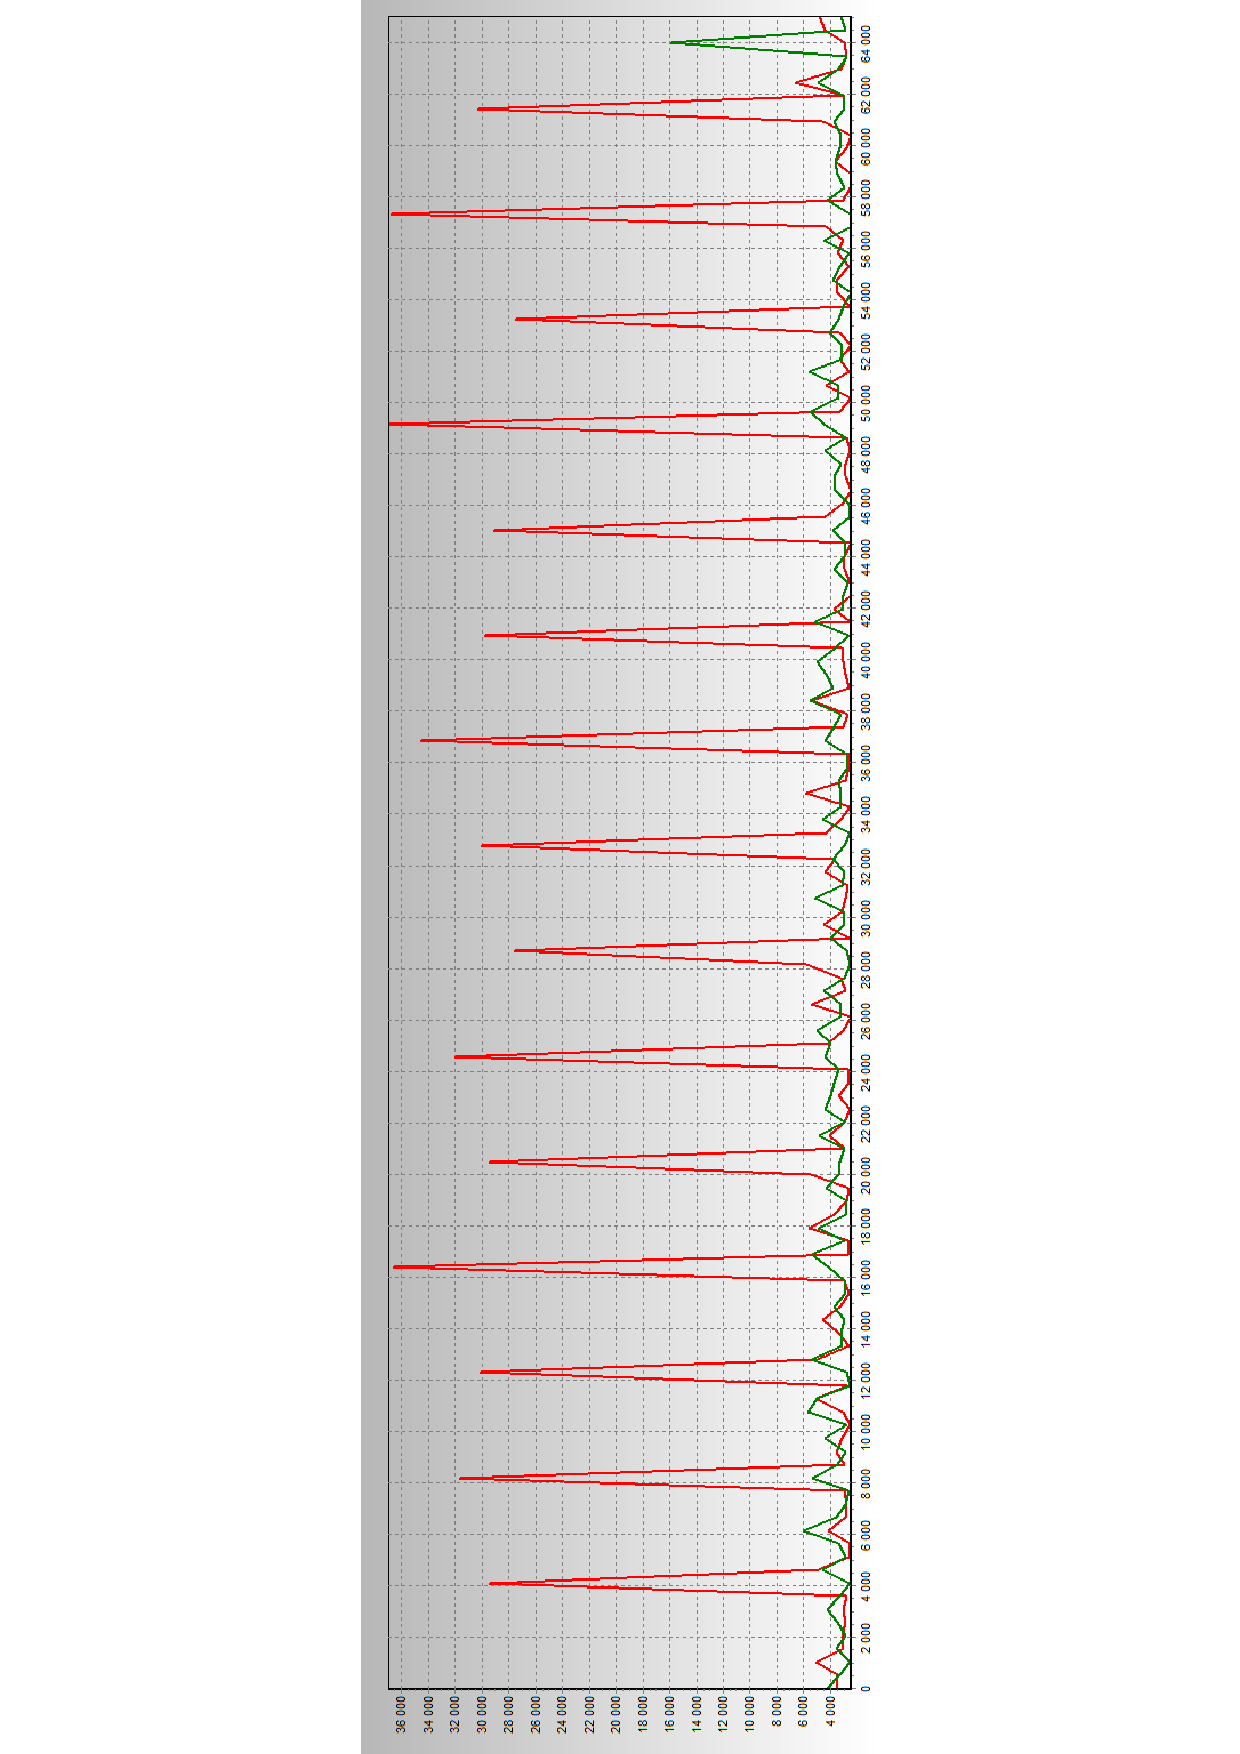
\includegraphics[width=0.7\textwidth, angle=90]{img/3.pdf}
	\label{img:3}
\end{figure}

Расстояние между пиками --- 4к. Пик --- работа с дескриптором --- преобразование в физический адрес.

\subsection*{Вывод}

Необходимо делать предвыборку заранее, если есть возможность.

\section{Эксперимент №4}

На рисунке \ref{img:4} представлен результат эксперимента.

\begin{figure}[H]
	\caption{График эксперимента 4}
	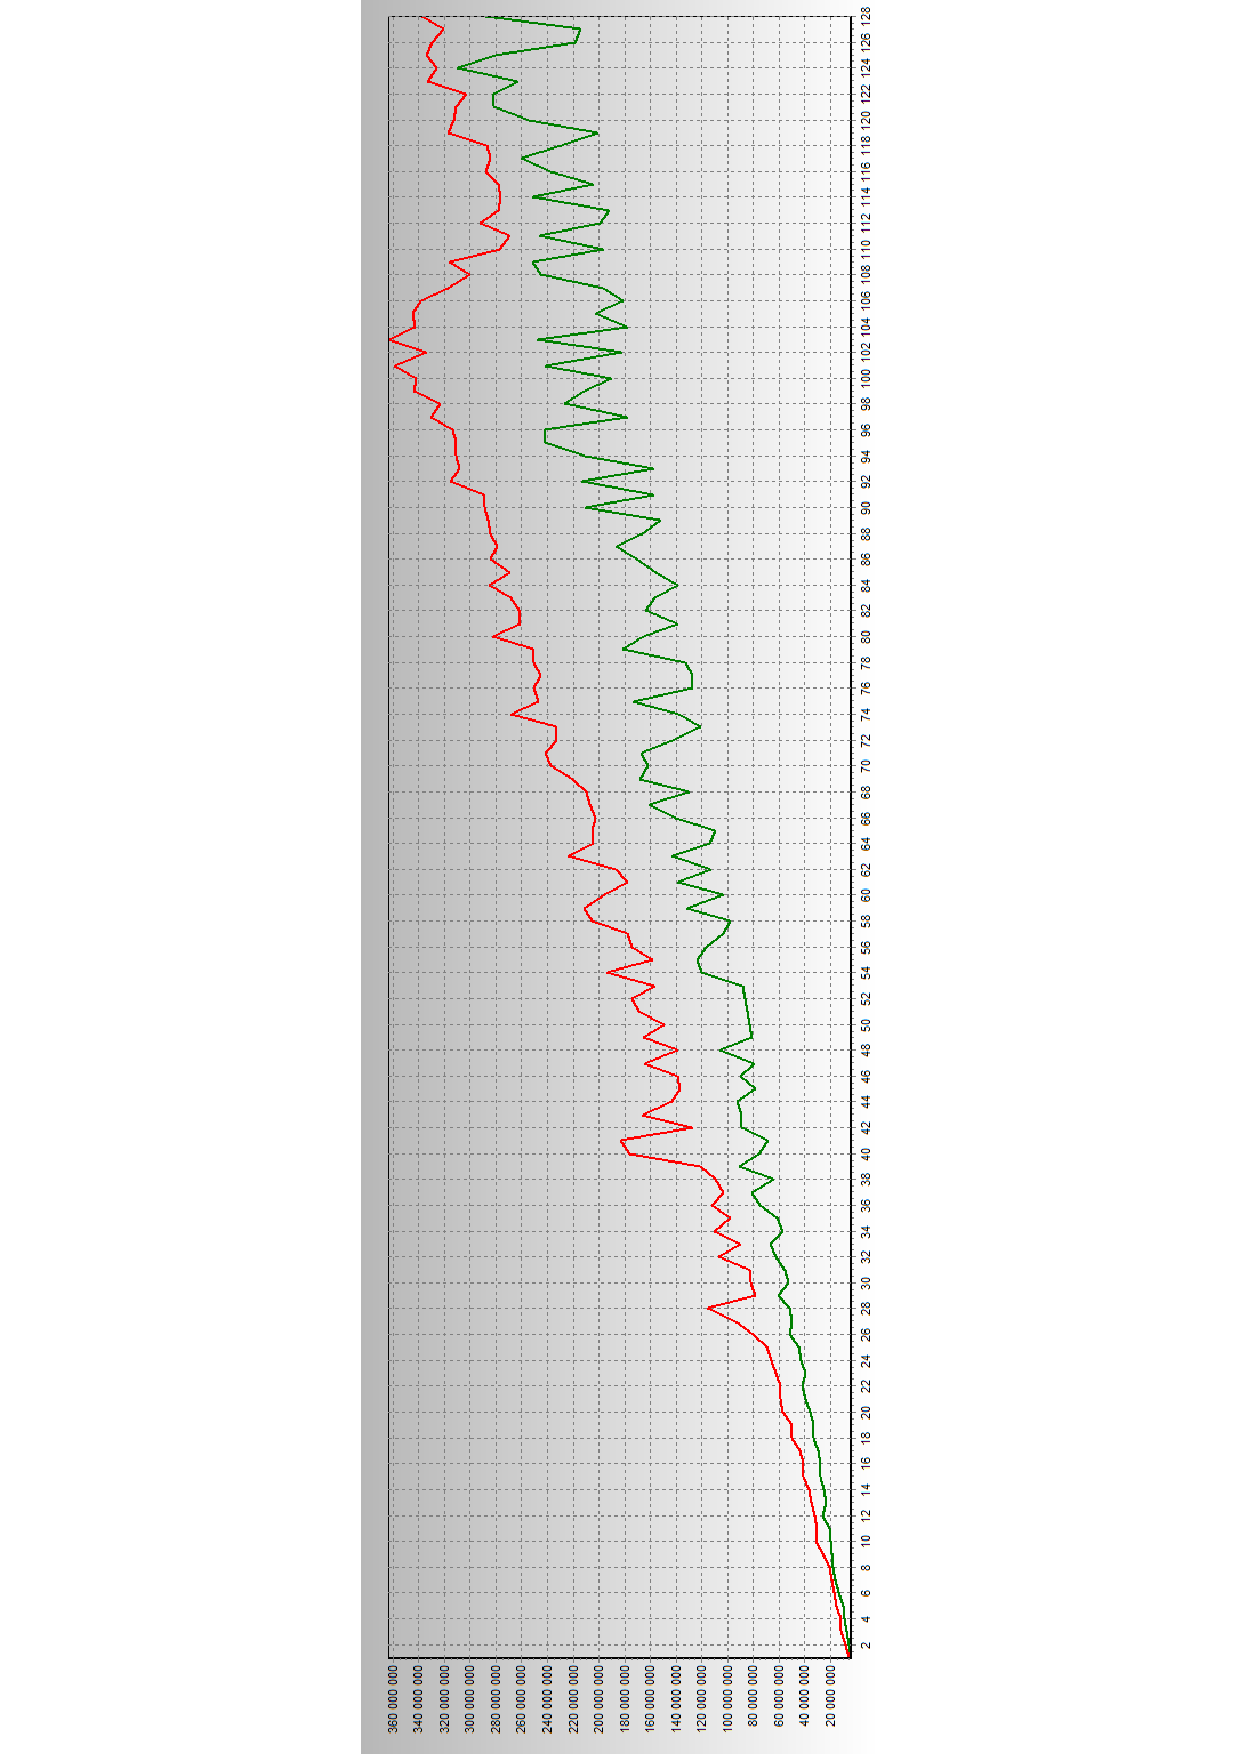
\includegraphics[width=0.7\textwidth, angle=90]{img/4.pdf}
	\label{img:4}
\end{figure}

\subsection*{Вывод}

Переход от массива структур к структуре массивов увеличивает эффективность обработки данных благодаря тому, что мы не отбрасываем результаты выборки, а используем все.

\section{Эксперимент №5}

На рисунке \ref{img:5} представлен результат эксперимента.

\begin{figure}[H]
	\caption{График эксперимента 5}
	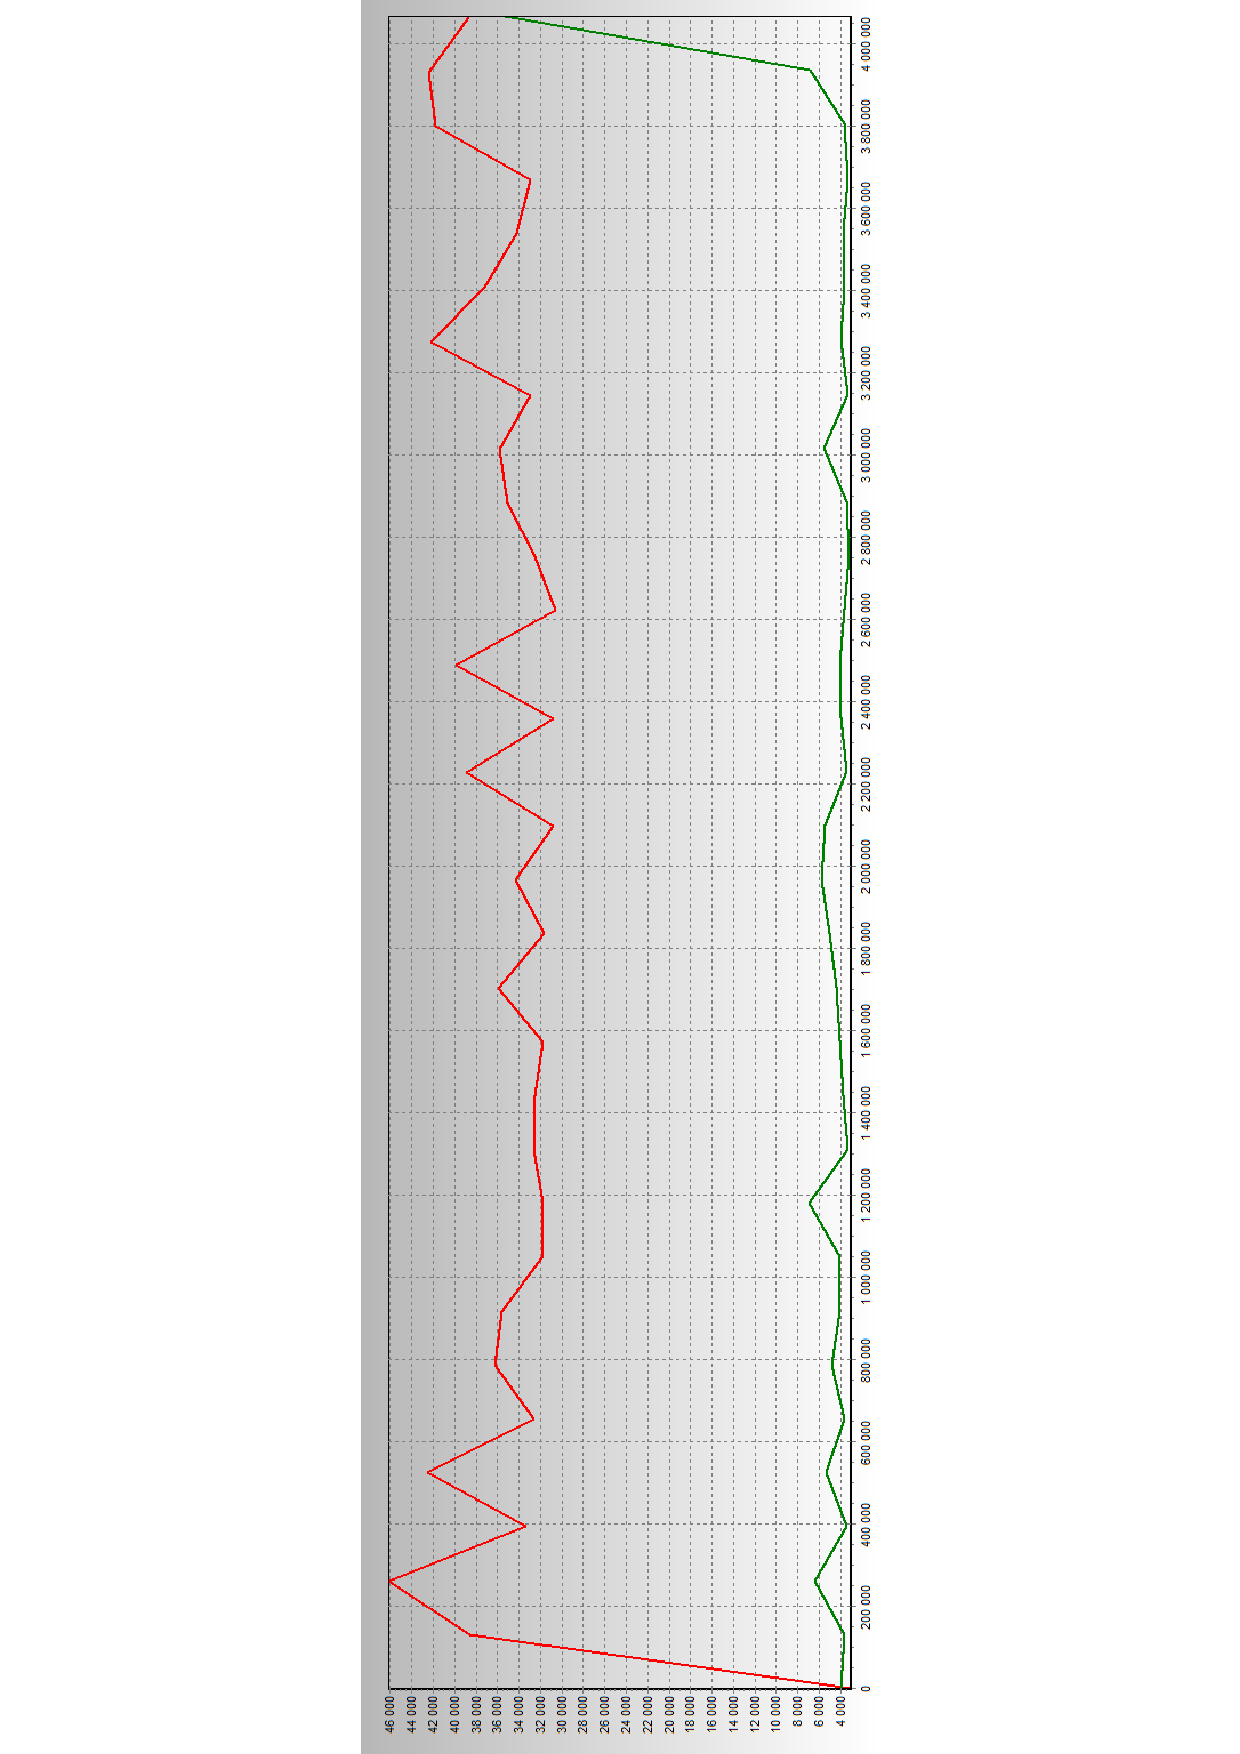
\includegraphics[width=0.7\textwidth, angle=90]{img/5.pdf}
	\label{img:5}
\end{figure}

\subsection*{Вывод}

Конфликты памяти замедляют работу всей системы, наличие кэш памяти~---~ускоряет.